\chapter{Algorithm to optimize mobility management}
\label{chp:problem_statement}

This chapter describes the details and design considerations of the algorithm presented for solving the problem of optimal mobility management in narrow beam systems. The strategy operates separately for each user, optimizing for maximizing throughput and minimizing handover rate against the user's speed.
\section{High level overview}
Before going in-depth into the algorithm's workings, we present a high-level overview of the handover strategy, specifying the inputs and outputs of the system. Figure~\ref{fig:algo-overview} provides a high-level graphical algorithm overview. Section~\ref{subsec:algo_exp} explains each component in detail in the order of their execution.
\subsection{Inputs and Outputs of the Algorithm}
\subsubsection{Inputs}
\label{subsec:algo-input}
\begin{itemize}
    \item \textbf{User position:} Coordinates of the UE based on the localization method described in Section~\ref{sec:mod-user-loc}
    \item \textbf{User velocity:} Recorded by the UE as the change in position. 
    \item \textbf{Current Serving AP/Beam:} The current optical beam or RF AP serving the UE when the handover procedure is initiated.
    \item \textbf{RSRP report:} An array storing the RSRP measurements recorded by the user for every available optical beam which can be detected by the UE and the RF AP
\end{itemize}
\subsubsection{Outputs}
The algorithm generates a single output:
\begin{itemize}
    \item \textbf{Choice:} the specific AP which the user needs to be switched to to maintain consistent connectivity with the network.
\end{itemize}
\subsection{Components of the Algorithm}
Broadly, the operations taking place during a single run of the algorithm can be categorized into the following phases:
\begin{itemize}
    \item \textbf{Handover Trigger:} This step specifies the preconditions for the handover to take place. It is also the step where the inputs necessary for the handover are derived or extracted from the UE.
    \item \textbf{Initialization Phase:} This step specifies the setup of certain parameters which dictate the behavior of the algorithm for this run. In addition, this step also initializes particular variables.
    \item \textbf{Prediction Phase:} This step specifies the operations that take place at each time-step across the prediction window. UE position is estimated based on which SINR is predicted. This predicted SINR is then used for evaluating the viability of all the optical beams/ RF APs for connection.
    \item \textbf{Decision Phase:} After predictions have been made for every time step within the prediction window, the decision phase then evaluates the score accrued by each Optical beam/ RF AP and makes the final choice of which Optical beam/ RF AP to connect the UE to.
\end{itemize}
\begin{figure}
    \centering
    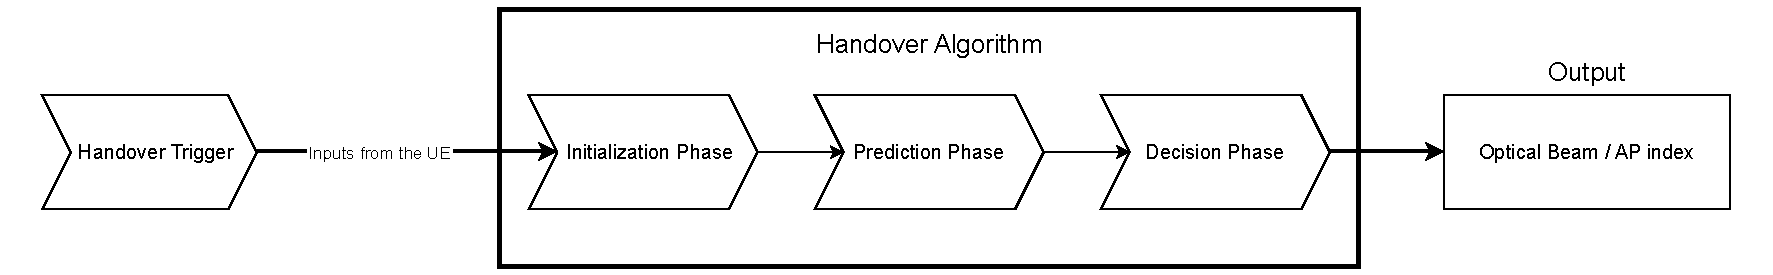
\includegraphics[width=1\linewidth]{Figures/Algorithm-design-High level overview.drawio.pdf}
    \caption{High-level overview of the phases of the algorithm}
    \label{fig:algo-overview}
\end{figure}

% \subsection{Sub-components}
% The workings of the algorithm are broadly classified into a pre-process and two consecutive blocks:
% \begin{itemize}
%     \item \textbf{Handover trigger:} Pre-conditions reported by the UE to the network with inputs as described in section~\ref{subsec:algo_overview} which trigger the handover strategy.
%     \item \textbf{Initialization of parameters:} Initialization of meta-parameters dictating the characteristics of a specific instance of the handover decision.
%     \item \textbf{Prediction phase:} The algorithm makes predictions 
%     \item Decision phase
\label{subsec:algo_overview}
\section{Detailed explanation}
\label{subsec:algo_exp}
\subsection{Handover trigger}
The handover algorithm follows a trigger-based strategy. This means that the handover process is only initiated when specific events occur or conditions are fulfilled. In this case, the specific trigger for initiating a handover is when RSRP measurements by the UE indicate that non-serving optical beam/RF AP is providing a higher SINR than that of the current serving optical beam or RF AP. The optical and RF networks periodically send reference signals, which are then utilized to calculate the RSRP measurements. The reference signals sent by the optical network also allow for the UE location to be tracked. The centers of the 3 beams providing the highest SINRs act as the end points for triangulation. Since the reference signals are sent continuously with a set period interval, a change in location between two consecutive measurements can be used to derive the velocity of the UE. The UE sends the RSRP measurements back to the network as an RSRP report. The network utilizes the UE measurement report to derive the most up-to-date location, velocity, and acceleration values. It then decides whether a handover process should be initiated. Figure~\ref{fig: handover-trigger} provides a graphical explanation of the handover trigger process.
% 
\begin{figure}
    \centering
    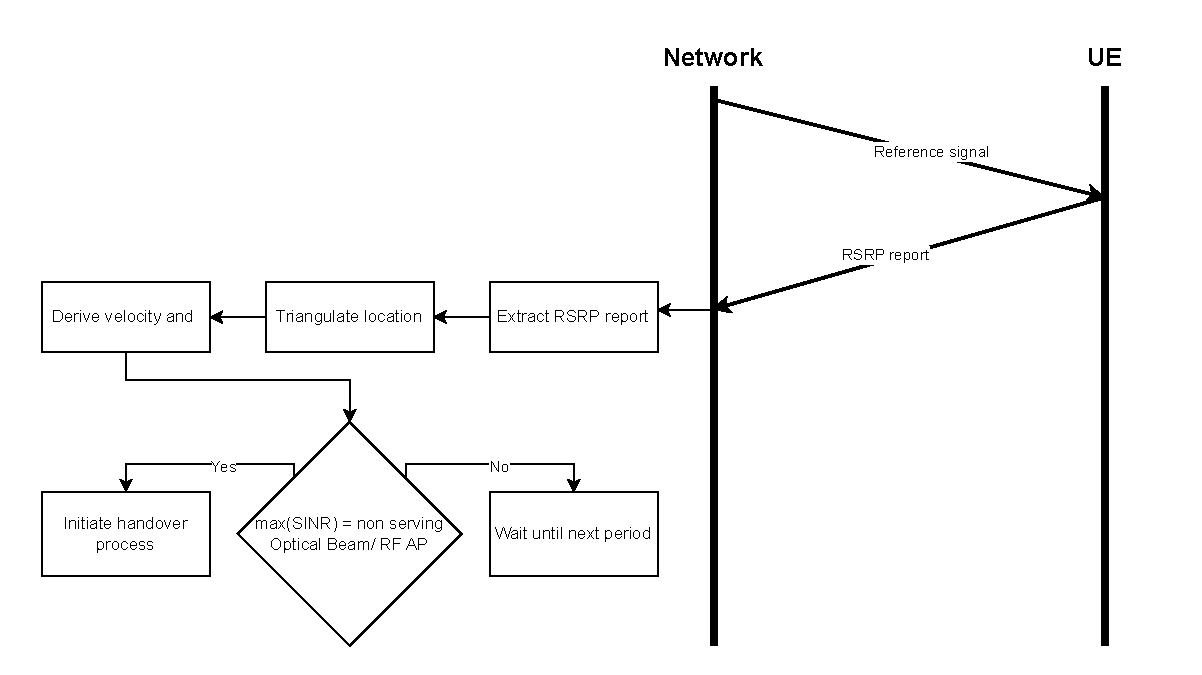
\includegraphics[width=1\linewidth]{Figures/Algorithm-design-Handover-trigger.drawio.pdf}
    \caption{Flowchart describing the handover trigger process}
    \label{fig: handover-trigger}
\end{figure}

\subsection{Parameters of the algorithm}
\label{subsubsec:param_init}
We first perform setup for certain parameters characterizing a specific instance of the handover algorithm. These parameters together impact and define the behavior of the selection logic:
\begin{enumerate}
    \item \textbf{Network selection coefficient $\lambda$:} Beyond a certain velocity of the user, it is no longer feasible for the optical network to adequately keep up with the user and provide consistent connectivity. In such situations, the algorithm must switch the UE to the RF Network. This is mathematically modeled by the network selection coefficient. It is a scalar that indicates the system's preference for the RF network over optical. Higher the velocity of the user, the higher is the value of the scaler.
    \item \textbf{Prediction window size $\eta$:} Vertical handovers require more time to perform due to the change in transmission interface. As such, the algorithm must be sure that it would still be most optimal for the user to be connected to the RF network by the time the handover completes. The prediction window size provides a dynamic way of adjusting how far in advance the algorithm will make estimations before making a decision. Vertical Handovers require a larger window size than horizontal handovers. 
\end{enumerate}
\subsection{Initialization phase}
When a handover condition is triggered, certain variables in the algorithm are initialized first. These are as follows:
\begin{enumerate}
    \item \textbf{Current step $k:$} For window size $\eta$, let $k$ represent the individual time-slot within the window where $1 \leq k \leq \eta$ and $k$ starts at 1. 
    \item \textbf{Current time $t_k:$} represents the time recorded at the start of the k-th step 
    \item \textbf{Prediction step size $t_{TTT}:$} Specifies the time interval between two consecutive predictions
    \item \textbf{Score:} Score is an array that keeps track of the SINR measurements throughout the execution of the algorithm. It is analyzed in the decision phase to determine which AP/beam to switch the user to. Let $\alpha$ and $\beta$ represent the total number of Optical beams and the total number of RF APs in the system. Thus, Score is an array of length $(\alpha + \beta)$. Optical beams are identified by index $i \in [0, \alpha)$ while RF APs are identified by the index $i \in [\alpha, \alpha + \beta)$. Score is initialized as a null array containing all zeroes.
    \item \textbf{Decay constant d:} The further the algorithm moves in the future, the more dependent the location estimation becomes on previous predictions. In turn, the probability of the location estimation deviating from ground reality increases. To compensate for such a potential error, We utilize exponential decay on the score per timeslot. Thus, as the predictions move further in the future, their impact on the score and thus the final decision reduces as well. To optimize the vertical handover process, it is necessary to adjust the decay constant $d$ in conjunction with the prediction window size. This adjustment aims to identify the optimal combination that allows for sufficient foresight into future events while appropriately weighting these future predictions. The goal is to ensure that these predictions neither exert zero influence on the final outcome nor have the same level of impact as more accurate, near-term predictions.
\end{enumerate}
\subsection{Prediction phase}
As long as we have not iterated through the entire prediction window $(k < \eta)$, for each slot we do the following:
\begin{enumerate}
    \item Predict the location at the $k+1$th slot. The short-term prediction is given by (\ref{eq:algo_pred-loc}). Here, $v(t_k)$ and $a(t_k)$ represent the derived velocity and acceleration of the UE in slot $k$ respectively.
    \begin{equation}
        p(t_k + t_{TTT}) \leftarrow p(t_k) + v(t_k) \times t_{TTT} + \frac{1}{2}a(t_k) \times t_{TTT}^2.
        \label{eq:algo_pred-loc}
    \end{equation}
    \item \textbf{SINR Estimation:} Based on the predicted location, the algorithm makes an estimate of the SINR from each optical beam/RF AP. 
    \item \textbf{Measurement adjustment: } The SINR from the RF AP is scaled by the network selection coefficient as shown in (\ref{eq:algo_measurement-scale}). Here, $\gamma$ represents the adjusted value while $\lambda$ is the network selection coefficient.
    \begin{equation}
        \gamma = 
\begin{cases} 
\text{SINR} \quad &\text{for optical beam} \\
\lambda \times \text{SINR} \quad &\text{for RF AP}
\end{cases}
\label{eq:algo_measurement-scale}
    \end{equation}
    \item \textbf{Score update:} The score array is updated as shown in (\ref{eq:algo_score_update}). Here, $\gamma$ is the adjusted measurement, $d$ is the decay constant and, $k$ is the current time slot. $\alpha$ and $\beta$ represent the total number of optical beams in the system and the total number of RF APs, respectively. 
    \begin{equation}
        Score[i] \leftarrow Score[i] + \gamma_i \times e^{-dk} \quad \text{for each } i \in [0, \alpha + \beta). 
        \label{eq:algo_score_update}
    \end{equation}

\end{enumerate}
Figure~\ref{fig:algo-prediction} showcases an overview of operations that take place in each time slot of the prediction window.
\begin{figure}
    \centering
    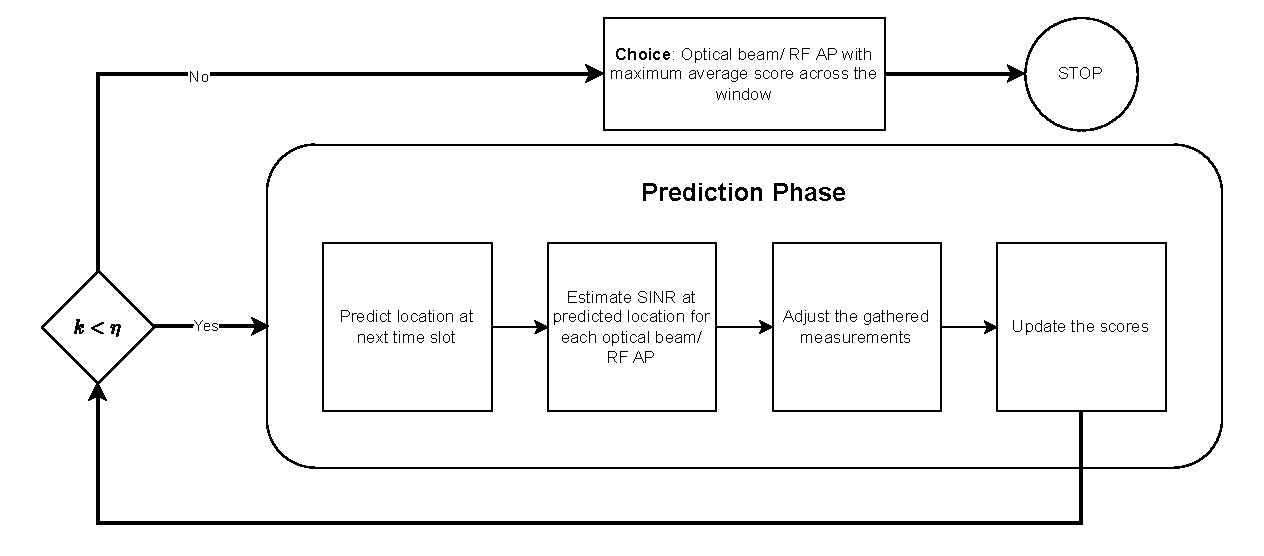
\includegraphics[width=1\linewidth]{Figures/Algorithm-design.drawio.pdf}
    \caption{Prediction phase of the algorithm: General summary of operations}
    \label{fig:algo-prediction}
\end{figure}
\subsection{Decision phase}
Once the prediction phase has been carried out for each slot in the prediction window, the algorithm decides on which AP to connect the user to. The algorithm selects the AP with the greatest score across the entire prediction window as given by (\ref{eq:algo-decide}). Here $\alpha$ and $\beta$ represent the total number of Optical beams and the total number of RF APs as defined previously in Section\ref{subsubsec:param_init}. 
\begin{equation}
        {choice} = \arg \max({Score}[i] \quad \forall i \in [0, \alpha + \beta)).
        \label{eq:algo-decide}
    \end{equation}

\section{Pseudo code}
Combining the individual components, we present a unified algorithm for both horizontal as well as vertical handovers as described by Algorithm ~\ref{alg:handover-complete}
\begin{algorithm}
\caption{Hybrid Handover Algorithm}
\label{alg:handover-complete}
\begin{algorithmic}[1]
\REQUIRE UE position, UE velocity, UE acceleration, Current serving AP/Beam
\ENSURE Choice (A specific optical beam / RF AP)

\STATE Initialize network selection coefficient $\lambda$ based on UE velocity
\STATE Set prediction window size $\eta$
\STATE $t_k \leftarrow$ current time
\STATE $t_{TTT} \leftarrow$ interval between two consecutive time slots
\STATE Score $\leftarrow$ array of zeros (size of num of optical beams + num of RF APs)
\STATE Decay constant $d$

\WHILE{$k < \eta$}
    \STATE Predict location at the $k+1$th slot
    \[
    p(t_k + t_{TTT}) \leftarrow p(t_k) + v(t_k) \times t_{TTT} + \frac{1}{2}a(t_k) \times t_{TTT}^2.
    \]
    \STATE Estimate SINR based on predicted location
    \STATE Adjust the estimated measurements:
    \[
    \gamma = 
    \begin{cases} 
    \text{SINR} \quad &\text{for optical beam} \\
    \lambda \times \text{SINR} \quad &\text{for RF AP}
    \end{cases}
    \]
    \STATE Update the score 
    \[
    \text{Score}[i] \leftarrow \text{Score}[i] + \gamma_i \times e^{-dk} \quad \text{for each } i \in [0, \alpha + \beta)
    \]
    \STATE $k \leftarrow k + 1$
    \STATE $t_k \leftarrow t_k + t_{TTT}$
\ENDWHILE

\STATE Choice $\leftarrow \arg \max\left(\text{Score}[i] \quad \forall i \in [0, \alpha + \beta)\right)$

\RETURN Choice (A specific optical beam / RF AP)
\end{algorithmic}
\end{algorithm}
% Define models with math, such that
% %
% \begin{equation}
% x = a^2 + b^2,
% \label{eq:EQUATION}
% \end{equation}
% %
% where $a$ and $b$ are your parameters, define your system.

% Remarks on style:

% \begin{enumerate}
% 	\item use `Section` name to refer to sections when citing (so Section~\ref{sec:SECTIONTITLE} not Sec.~\ref{sec:SECTIONTITLE} or section~\ref{sec:SECTIONTITLE}); Same comment applies to Tables, Algorithms and Figures
% 	\item Tables and figures must be at the top of the page---use [t] marker (not [h], for `here`); 
% 	\item Every caption should end with a period;
% 	\item Encapsulate equations in `()` brackets and do not add word `equation before` (therefore `in~(\ref{eq:EQUATION})`, not `in Equation~\ref{eq:EQUATION}` or in Eq.~\ref{eq:EQUATION});
% 	\item Equations are sentences, so punctuation applies at the end of it (comma, semicolon or full-stop).
% \end{enumerate}

% Here is a simple table

% \begin{table}[t]
% \centering
% \begin{tabular}{| l | c | r |}
% \hline
% left aligned & centred & right aligned \\
% \hline \hline
% 12 & 34 & 56 \\
% \hline
% \end{tabular}
% \caption{Complete sentence describing the tabular data. Caption should summarize the conclusions of the result.}
% \label{tab:table_1}
% \end{table}

% Here is a simple figure.

% \begin{figure}[t]
% \includegraphics[width=\textwidth]{template-pics/tud-es-logo-tikz/tud-es-logo}
% \caption{Complete sentence describing the figure thoroughly. Caption should summarize the conclusions of the result.}
% \label{fig:example-figure}
% \end{figure}

% Citations are here~\cite{polastre2004analysis,powercast_website,hester2016persistent,schaper_msc_thesis_2017,dementyev_uist_2016}. See `bib/MyMScTUDESThesisBibFile.bib` file for a list of requirements when typesetting a bibliography.
